\subsection{Gateway}
This section we will be detailing our plans for incorporating a LoRaWAN gateway into our design. We will not be designing the hardware in the same way that we are designing the hardware for the sensor node i.e. designing the PCB, etc., but we will need to build a functioning LoRaWAN gateway in order for sensor node to be useful. This section will focus on what we will need to do to set up the physical gateway components, which are a Raspberry Pi 4 and a RAK 2245 Pi Hat. We will also discuss how the software will need to be set up on the gateway in order to be able to connect it to our AWS instance using AWS IoT Core and The Things Network.

\subsubsection{Gateway Hardware}
The hardware assembly for the gateway is incredibly simple. All that needs to be done is to attach the RAK 2245's connector to the Raspberry Pi's 40-pin GPIO header. After this, it is simply a matter of connecting the Ethernet output to an internet router and plugging in the micro-USB cable for power. Additionally, the GPS antenna and the LoRa antenna that come with the RAK 2245 must be attached to it in order for the gateway to function. The only other component that is required is an SD card loaded with a Linux image developed by RAKWireless designed for the gateway. Our setup gateway can be seen is Figure \ref{fig:gateway-rak}.

\begin{figure}
    \centering
    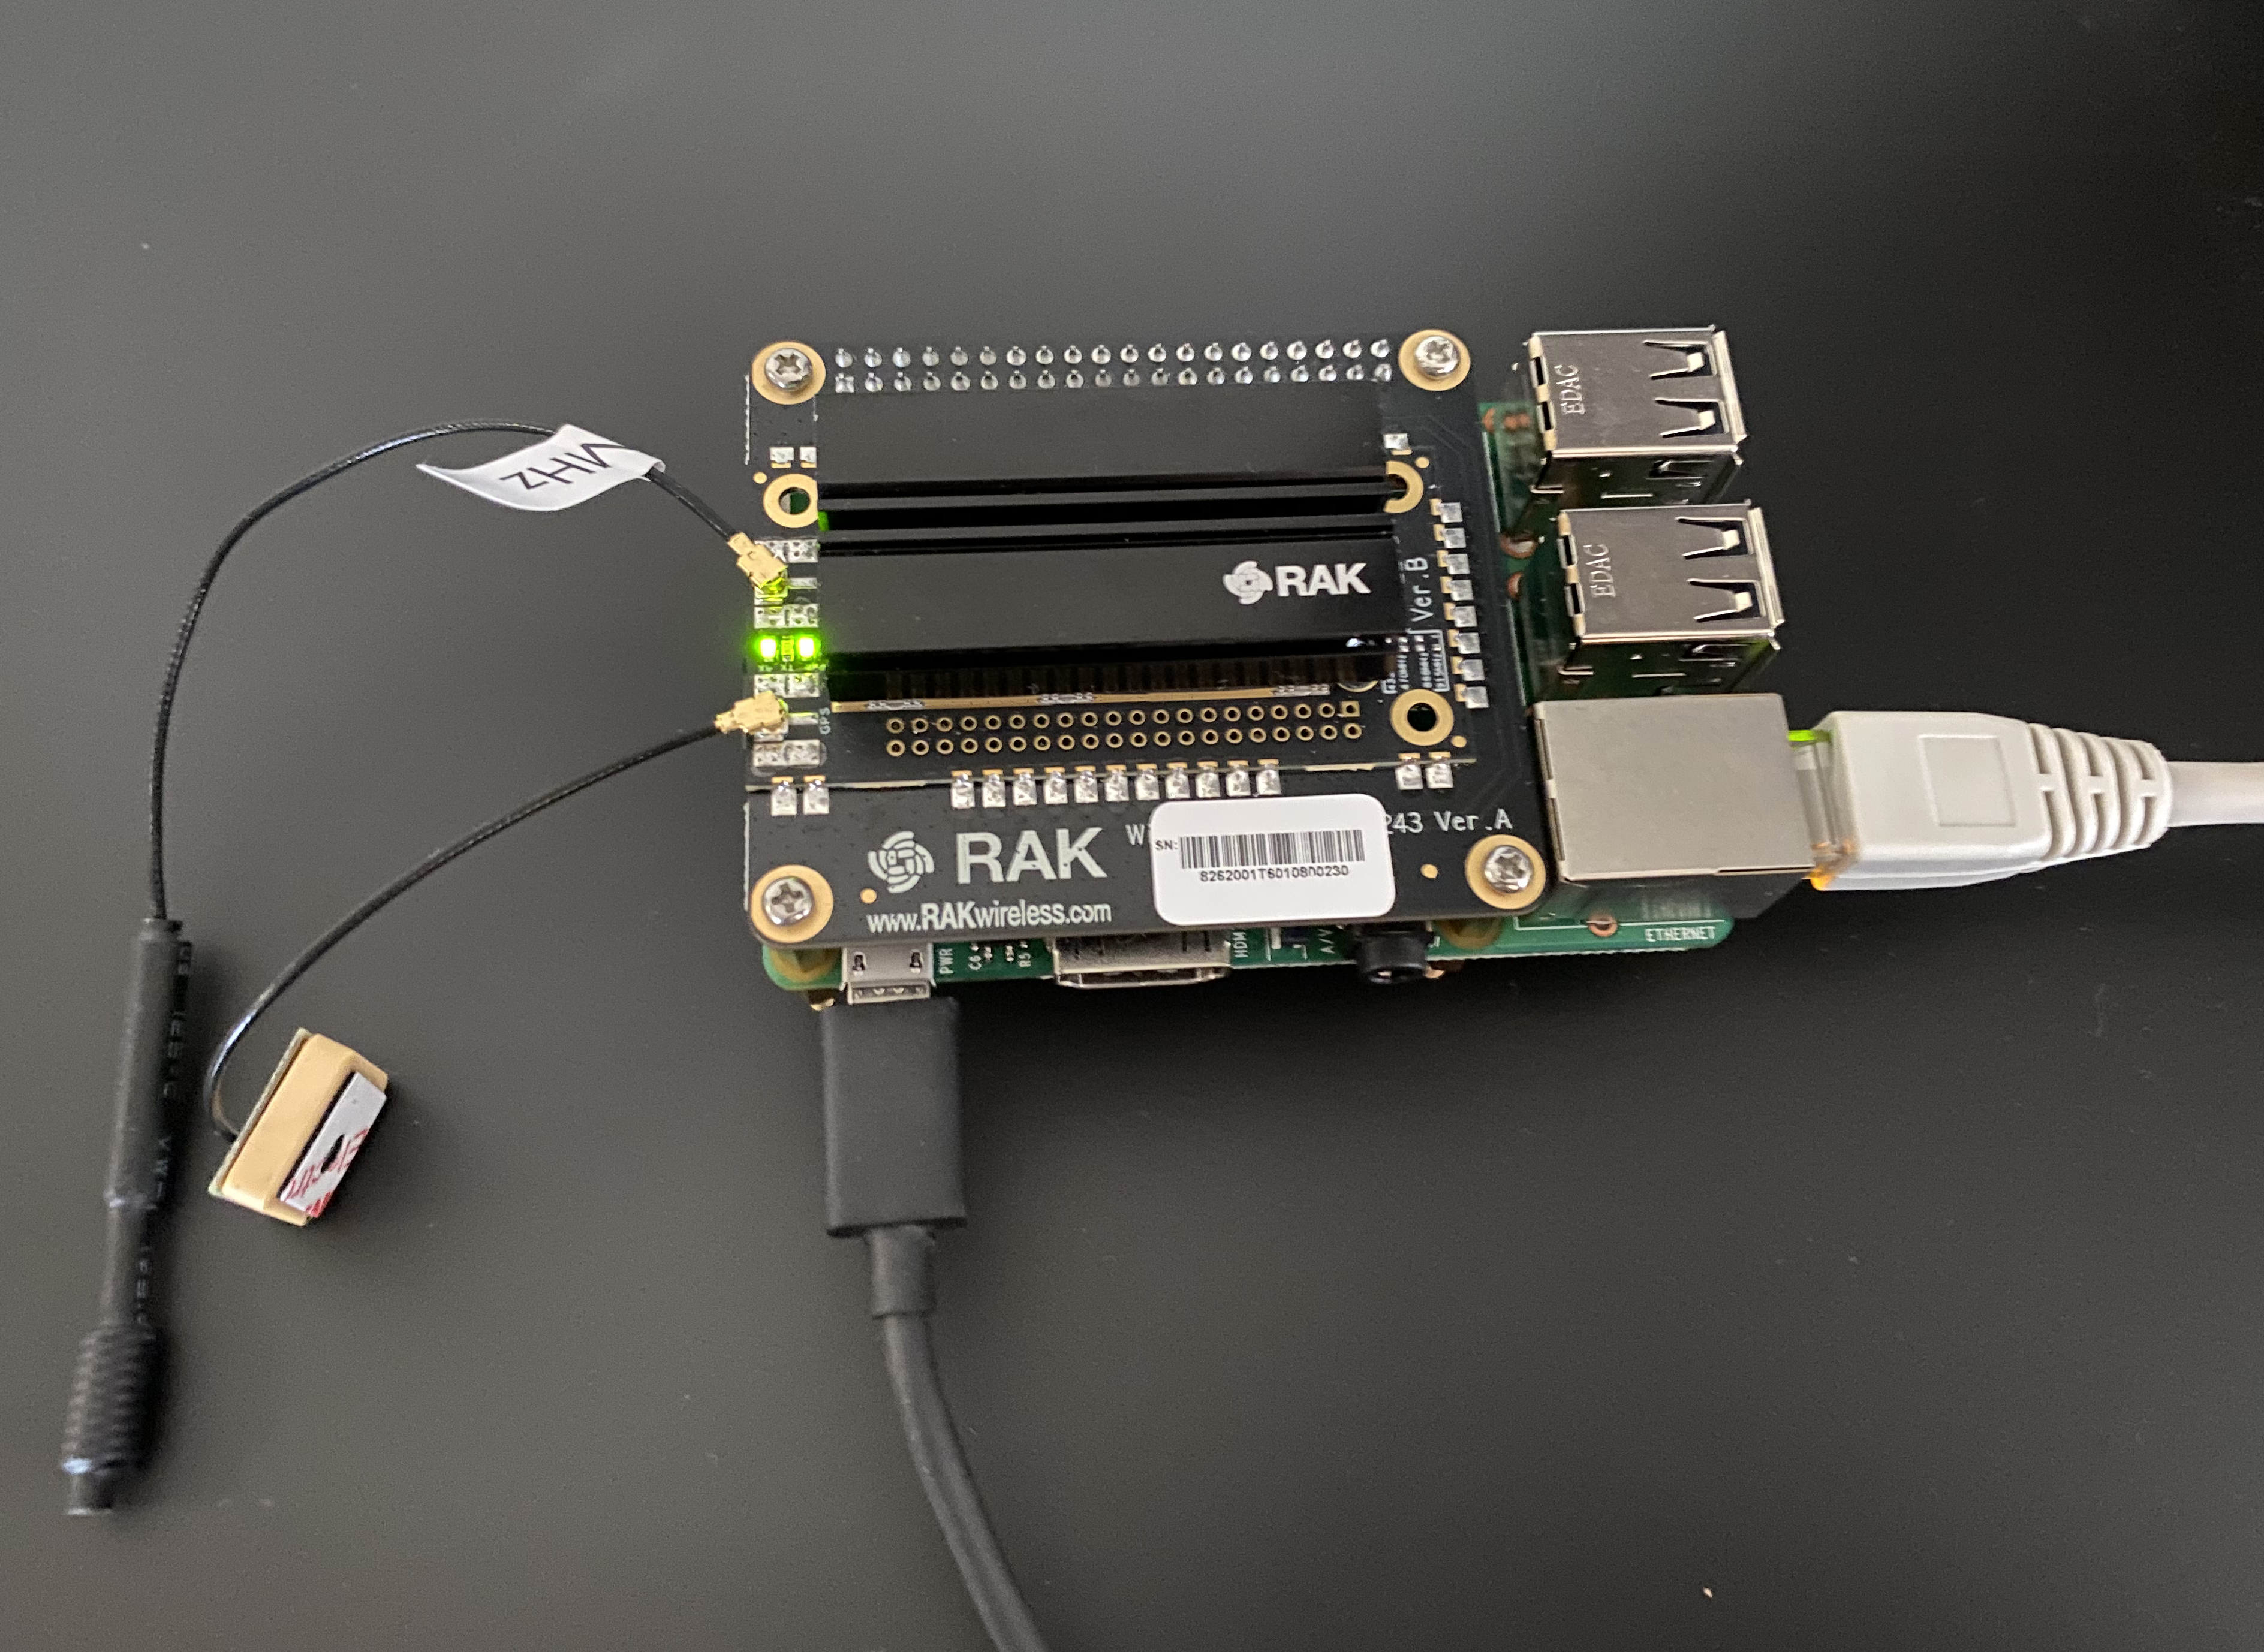
\includegraphics[width=4.5in]{figures/gateway-rak.png}
    \caption{An image of our setup gateway. It shows the Raspberry Pi 4 connected with the RAK 2245 Pi Hat.}
    \label{fig:gateway-rak} 
\end{figure}

\subsubsection{Gateway Software}
Configuring the gateway to function with the various LoRaWAN networks we desire is also fairly straightforward. Once we burn the previously mentioned OS image to an SD card and insert it into the Raspberry Pi, the device will create a new WiFi access point. On a separate computer, we will be able to connect to this WiFi access point and then can gain access to the gateway via an SSH connection. Within this SSH connection is where we will be able to configure that gateway to connect to any of the LoRaWAN networks we choose. In the next few sections we will detail how we will connect our gateway to The Things Network and directly to our AWS server instance.

\paragraph{Connecting to The Things Network}
Connecting to The Things Network is simply a matter of configuring the LoRaWAN gateway and using The Things Network's online configuration tool to add your gateway to the network.

To configure the gateway itself, one needs to connect to the gateway via SSH and then run the \texttt{gateway-config} command as follows. Also, run the \texttt{gateway-version} command. The information from this command will be used to add the gateway to the network.

\begin{tabular}{l}
     \texttt{\$ ssh pi@192.168.10.10} \\
     \texttt{\$ sudo gateway-config} \\
     \texttt{\$ sudo gateway-version} \\ 
\end{tabular}

This will bring up a menu GUI. In this menu, you select option 2, "\texttt{Setup RAK Gateway LoRa concentrator}. Then select the server plan, which is \texttt{Server is TTN}. Next, you select the appropriate region and frequency region, which in our case is \texttt{US\_902\_928}. After this, configuration on the device itself is finished. We will need to move to the Things Network's website next.

To finish setting up our gateway with The Things Network, we must navigate to The Things Network's website\footnote{The website for The Things Network is \texttt{www.thethingsnetwork.org}} and create an account. Once logged in, navigate to the Console, select your region, and then click "Add gateway." Once there, fill out the appropriate information for the gateway including the \texttt{Gateway ID} and appropriate frequency plan. After completing this, any LoRaWAN end-device that is correctly configured to connect to The Things Network should be able to see your newly setup gateway and use it to connect to the internet.

% \paragraph{The Helium Network}

\paragraph{Connecting Our AWS Server Instance}
Connecing our gateway to an AWS server instance will be somewhat similar to how we set it up to connect to The Things Network. It will require installing a custom operating system on the Raspberry Pi and performing some configuration on both the Pi and on AWS IoT Core, which is what we will be using to manage the gateway.

To begin configuring the Raspberry Pi, we are going to use Basic Station\footnote{The source code for Basic Station can be found at \texttt{https://github.com/lorabasics/basicstation}}, which is an open-source LoRaWAN gateway implementation. This will be installed on the Raspberry Pi. In order to use Basic Station with the RAK 2245, we have to make a few changes to the operating system. We must remove the following libraries:

\begin{tabular}{l}
     \texttt{\$ rm ./build-rpi-std/lib/liblgw.a} \\
     \texttt{\$ rm ./deps/lgw/platform-rpi/libloragw/libloragw.a} \\
\end{tabular}

We also need to modify the \texttt{SPI\_SPEED} variable from within the \\ \texttt{loragw\_spi.native.c} file. We are then ready to compile Basic Station by running the following command:

\begin{tabular}{l}
     \texttt{\$ make platform=rpi variant=std} \\
\end{tabular}

Once compiled, we have to create an \texttt{init.sh} script as well as directory to store configuration and credentials (keys, IDs, etc.) for AWS IoT Core. The code for the \texttt{init.sh} script is provided to us by AWS and is simply a matter of copying and pasting the script into the home directory of the Raspberry Pi. Creating the directory is just as simple as running \texttt{mkdir}. Once this is done, we will then run the \texttt{init.sh} script. We can then start Basic Station with the test server and credentials using the following command:

\begin{tabular}{l}
     \texttt{\$ cd \$HOME/basicstation/examples/live-s2.sm.tc} \\
     \texttt{\$ RADIODEV=/dev/spidev0.0 ../../build-rpi-std/bin/station} \\
\end{tabular}

We will use the output of these commands to determine our gateway's \texttt{EUI}. To begin the process of connecting our gateway to AWS IoT Core, we will navigate to the AWS IoT Core Management console. From there, we will click "Add a gateway." This is where will provide IoT Core with our gateway's \texttt{EUI}. Then, IoT Core will prompt us to generate gateways certificates. This will ensure that our gateway can connect to our server securely and verify it's identity. We will have downloaded the following files, which should then be copied to our Raspberry Pi and placed in the configuration directory we created earlier:

\begin{itemize}
    \item \code{nnnnnnnn-nnnn-nnnn-nnnn-nnnnnnnnnnnn.cert.pem} - This is the gateway device certificate file
    \item \code{nnnnnnnn-nnnn-nnnn-nnnn-nnnnnnnnnnnn.private.key} - This is the gateway device private key file
    \item \code{lns.trust} - This is the trust certificate for the LoRaWAN Network Server (LNS) endpoint
    \item \code{cups.trust} - This is the trust certificate for the CUPS endpoint
\end{itemize}

We will also need to rename the \code{.cert.pem} and \code{.private.key} files to \code{cups.crt} and \code{cups.key} respectively. Once all of this is completed, we should end up with the following files within our configuration directory:

\begin{itemize}
    \item \code{cups.trust}
    \item \code{cups.uri}
    \item \code{cups.crt}
    \item \code{cups.key}
    \item \code{station.conf}
    \item \code{version.txt}
\end{itemize}

We can then start up the Basic Station software using the command we ran earlier. At this point, the Basic Station software should begin to establish a connection AWS IoT Core for LoRaWAN. Additionally, if we have our end-device connected to AWS IoT Core, we should be able to see log entries every time the device is sending packets through the gateway.